\documentclass{standalone}
\usepackage{tikz}
\usetikzlibrary[arrows,positioning,matrix]

\begin{document}
\begin{tikzpicture}
  \node[draw=none] (averageposture) {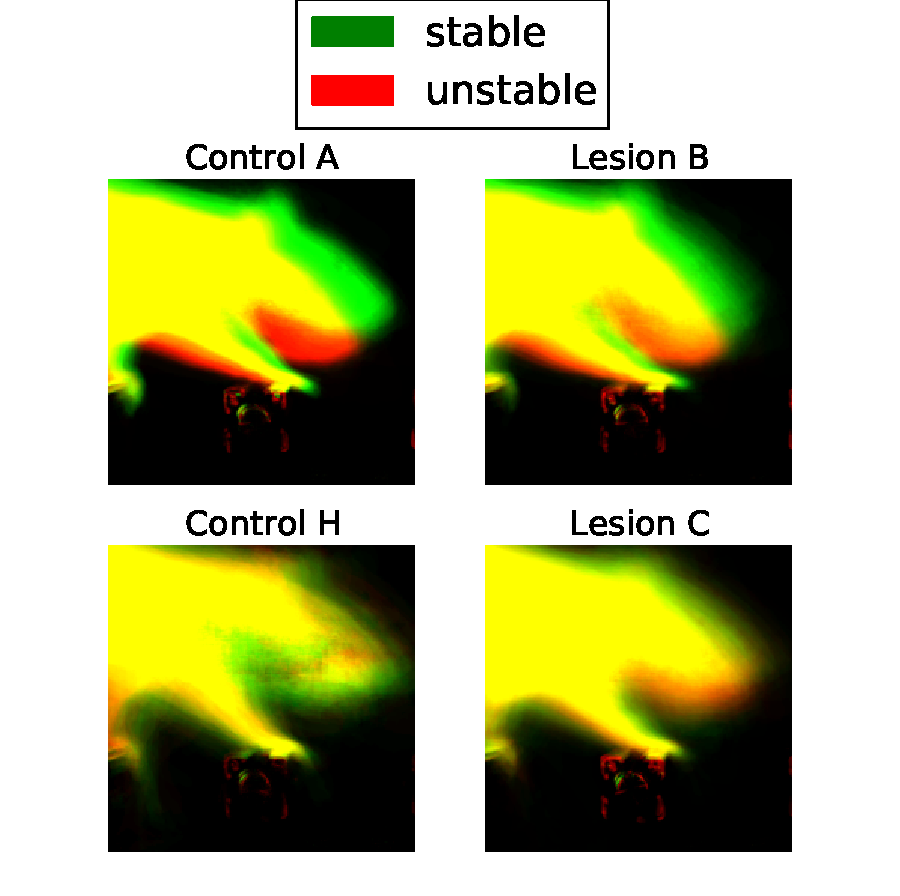
\includegraphics[width=0.33\textwidth]{elements/averageposture}};
  \node[draw=none,above left=-5mm of averageposture] (A) {A};

  \node[draw=none,right=1mm of averageposture] (jumptrajectory) {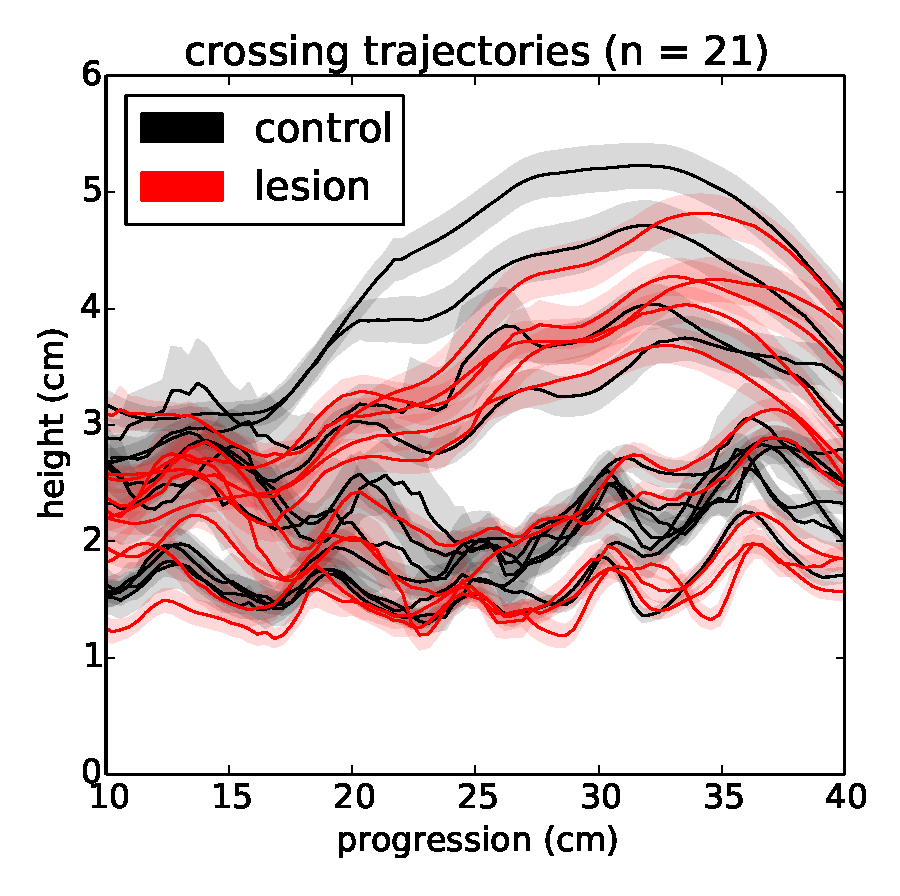
\includegraphics[width=0.33\textwidth]{elements/noseTrajectoryUnstable}};
  \node[draw=none,above left=-5mm of jumptrajectory] (B) {B};
  
  \node[draw=none,right=1mm of jumptrajectory] (jumpweight) {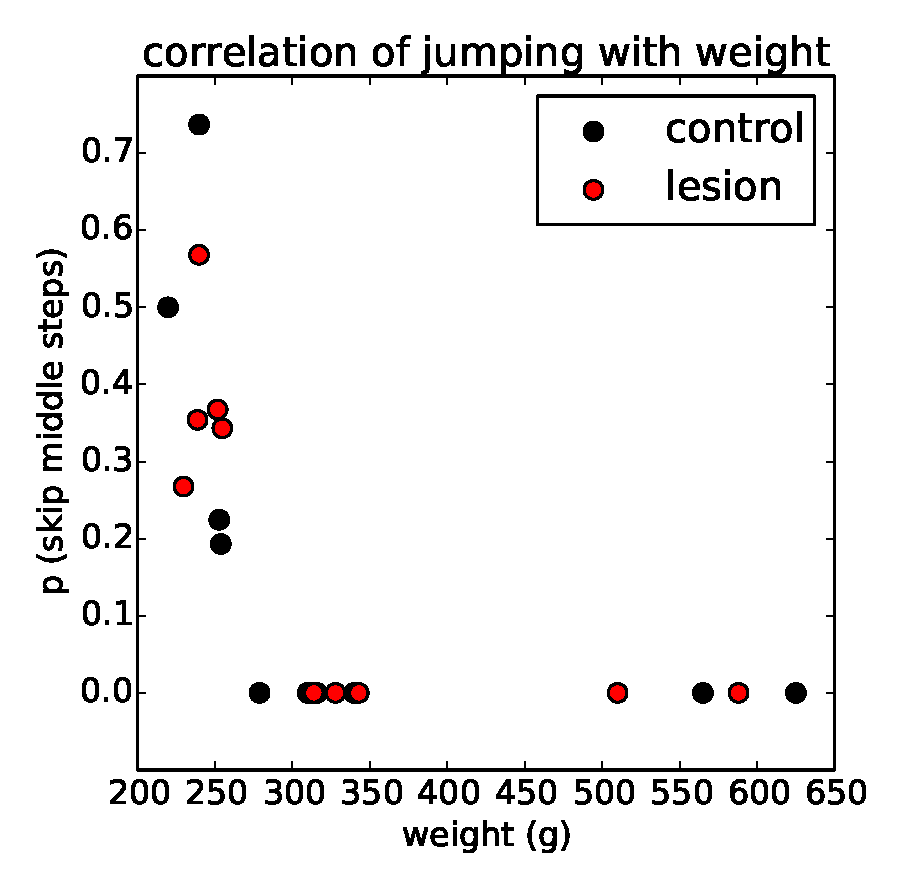
\includegraphics[width=0.33\textwidth]{elements/correlationJumperWeight}};
  \node[draw=none,above left=-5mm of jumpweight] (C) {C};
\end{tikzpicture}
\end{document}